% !TEX root = ../thesis.tex
%
\chapter{Application}
\label{sec:application}
\begin{figure}[h!]
    \begin{tabulary}{\textwidth}{cc}
        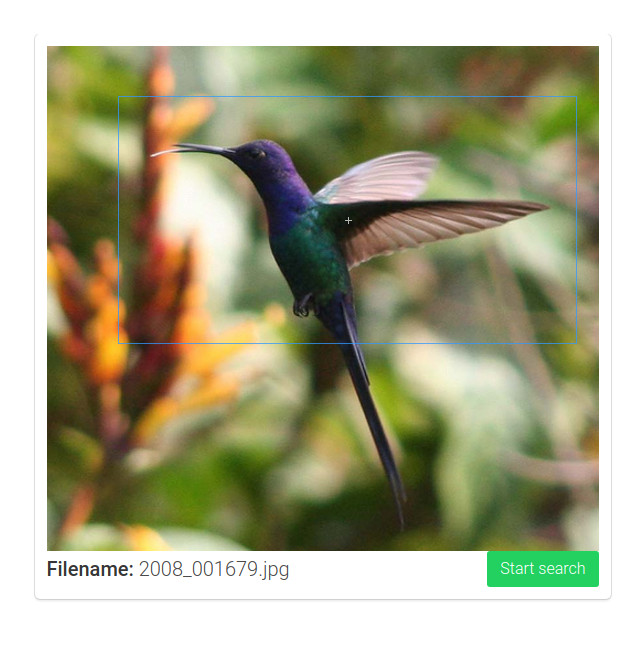
\includegraphics[height=4.5cm]{figures/server_select} &
        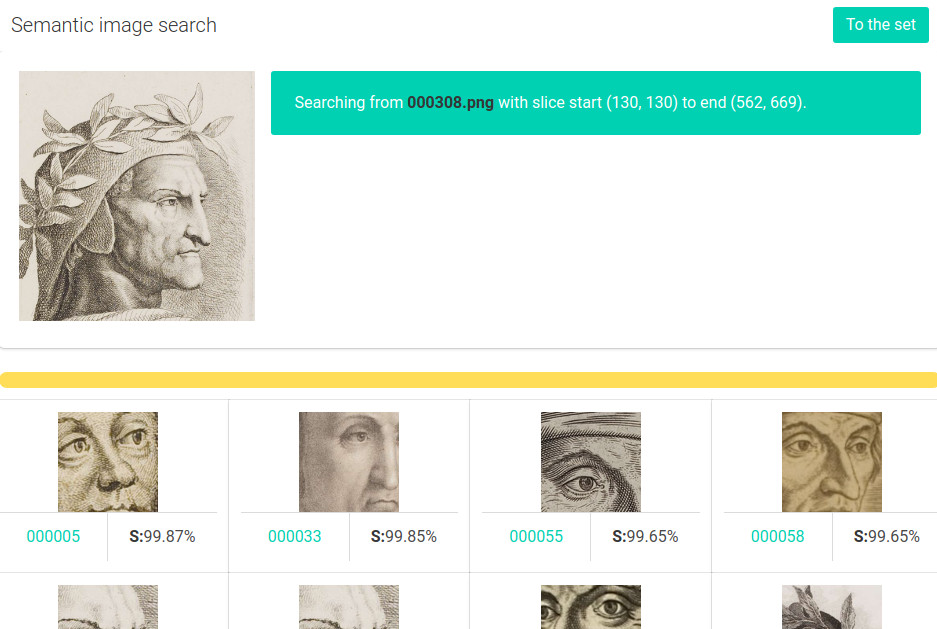
\includegraphics[height=4.5cm]{figures/server_results}
    \end{tabulary}
    \caption{Two screenshots of the provided online app using our method. Left shows the selection screen previous to a new search. Right shows the result screen displaying live results.}
    \label{fig:application}
\end{figure}
We bring the described method to application as a semantic image search machine. For this we build a small exemplar web application using the Flask microframework.

After configuring the program for a new image database, the web application enables users to search for similar objects given a query image patch. In the main view the user can sift through the image dataset to pick a image which contains the object of interest. For a single image the \gls{gui}\fref{fig:application} provides a simple graphical way to select a rectangular part of an image. Alternatively the user may upload an image to the web page, to search the database with an external image. Next the user can start the search with the provided patch. The backend quickly fine-tunes the \gls{resnet} under the same conditions as described in \treft{sec:results}.

Following the training, the network is instantly reshaped into the \gls{fcn} and set up for normal image forwarding. The images from the database are all forwarded through the detection pipeline. While the network is still running the program collects the best results and presents the patches with the highest score to the user, in descending order by their scores.

\TODO{examples of retrieval}
